
\chapter{Design and Architecture of Autonomous Vision-Enabled Delivery Vehicle for Smart Warehouse Applications}

The integration of autonomous robotics in warehouse operations represents a significant advancement in industrial automation, addressing the growing demand for efficient, accurate, and cost-effective material handling solutions. This chapter presents a comprehensive analysis of an autonomous delivery vehicle system that combines embedded systems, computer vision, robotic manipulation, and wireless communication technologies to create a self-operating warehouse assistant. The proposed system demonstrates how modern microcontroller platforms can be leveraged to build sophisticated autonomous vehicles capable of identifying, picking, transporting, and placing packages with minimal human intervention. The design emphasizes modularity, scalability, and real-time operational monitoring through cloud-based infrastructure, making it suitable for deployment in various warehouse environments.

\section{Contents of this Chapter}
This chapter provides a detailed examination of the autonomous delivery vehicle system through the following comprehensive sections:
\begin{enumerate}
\item System Specifications and Requirements
\item Pre-Analysis Work and Technology Selection
\item Detailed Design Methodology
\item System Architecture and Integration
\item Hardware Design Equations and Calculations
\item Software Architecture and Implementation Strategy
\item Communication Protocol Design
\item Testing and Validation Methodology
\end{enumerate}

\section{System Specifications and Requirements}

The autonomous delivery vehicle system is designed to meet the following technical specifications and operational requirements:

\subsection{Functional Requirements}
\begin{itemize}
\item \textbf{Autonomous Navigation}: The system must navigate warehouse environments using predefined paths and QR code checkpoints
\item \textbf{Object Recognition}: Real-time identification and classification of packages, items, and warehouse infrastructure
\item \textbf{Pick and Place Operations}: Precise manipulation of objects with varying sizes, shapes, and weights
\item \textbf{Wireless Communication}: Continuous connectivity with cloud-based monitoring systems
\item \textbf{Position Tracking}: Accurate location determination using QR code scanning and decoding
\end{itemize}

\subsection{Performance Specifications}
\begin{itemize}
\item \textbf{Operating Voltage}: 5V DC for motor systems, 3.3V for microcontroller operations
\item \textbf{Payload Capacity}: Up to 2kg for standard warehouse items
\item \textbf{Speed Range}: 0.1 - 0.5 m/s with PWM-controlled variable speed
\item \textbf{Arm Reach}: 300mm horizontal reach with 3-DOF articulation
\item \textbf{Vision Range}: 640x480 pixel resolution with 60-degree field of view
\item \textbf{Communication Range}: Wi-Fi connectivity within 100m of access points
\end{itemize}

\subsection{Environmental Specifications}
\begin{itemize}
\item \textbf{Operating Temperature}: 0°C to 50°C
\item \textbf{Humidity}: 10\% to 85\% non-condensing
\item \textbf{Surface Compatibility}: Smooth concrete floors with minimal debris
\item \textbf{Lighting Conditions}: Standard warehouse lighting (200-500 lux)
\end{itemize}

\section{Pre-Analysis Work and Technology Selection}

\subsection{Microcontroller Platform Analysis}
The selection of the NodeMCU ESP8266 as the central processing unit was based on comprehensive analysis of available microcontroller platforms. The ESP8266 offers several advantages for this application:

\begin{itemize}
\item \textbf{Integrated Wi-Fi}: Built-in wireless connectivity eliminates the need for additional communication modules
\item \textbf{Processing Power}: 80MHz Tensilica L106 32-bit RISC processor provides sufficient computational capability
\item \textbf{Memory}: 128KB RAM and 4MB Flash memory support complex program execution
\item \textbf{GPIO Availability}: 17 GPIO pins accommodate motor control, servo control, and sensor interfaces
\item \textbf{Cost Effectiveness}: Low-cost solution suitable for scalable deployment
\end{itemize}

\subsection{Motor Control System Analysis}
The L298N dual H-bridge motor driver was selected based on the following criteria:
\begin{itemize}
\item \textbf{Dual Channel Operation}: Simultaneous control of two DC motors for differential drive
\item \textbf{Current Capacity}: 2A per channel supports standard DC gear motors
\item \textbf{PWM Compatibility}: Direct interface with ESP8266 PWM outputs
\item \textbf{Protection Features}: Over-temperature and over-current protection
\end{itemize}

\begin{figure}[H]
    \centering
    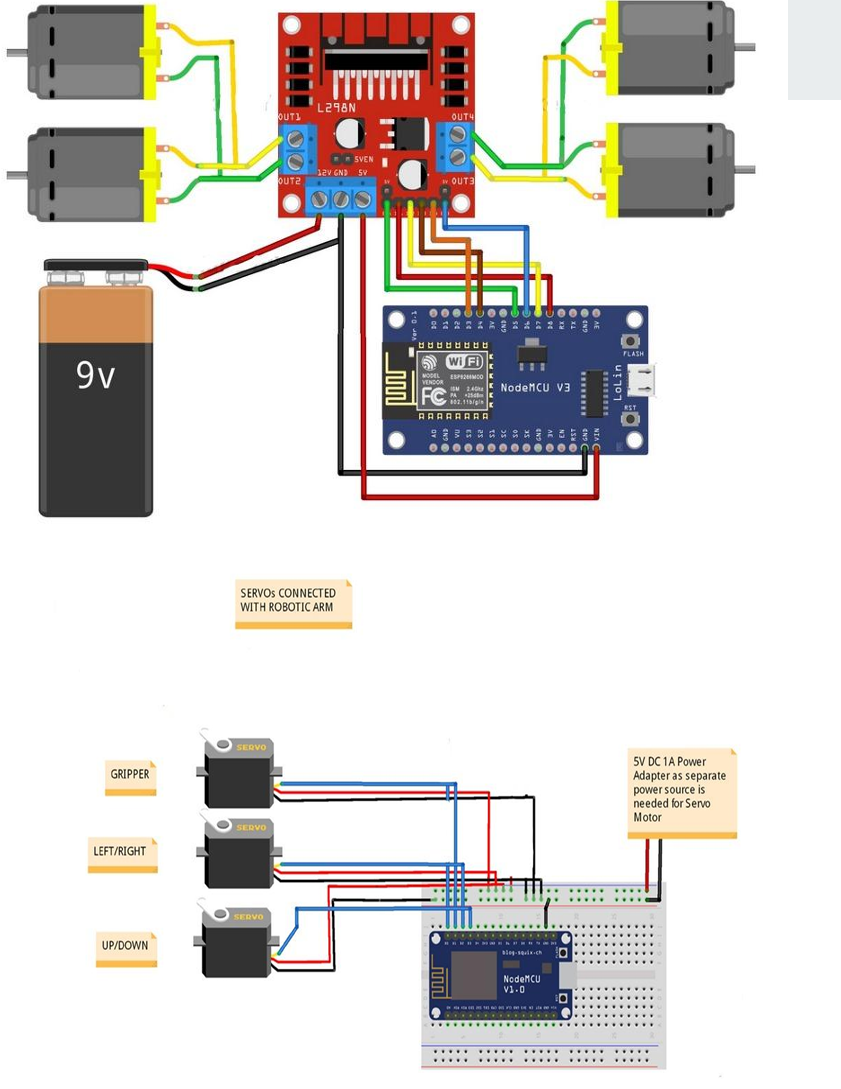
\includegraphics[width=0.9\textwidth]{./Chapter3/Figures/circuit_diagram.png}
    \caption{Circuit Diagram}
    \label{fig:architecture}
\end{figure}

\subsection{Vision System Technology Selection}
The integration of camera-based vision with the LLaMA-4 model provides advanced object recognition capabilities:
\begin{itemize}
\item \textbf{Real-time Processing}: On-device image capture with cloud-based analysis
\item \textbf{Multi-modal Recognition}: Combined visual and contextual understanding
\item \textbf{Adaptability}: Learning capability for new object types and warehouse layouts
\item \textbf{Accuracy}: High-precision object identification and classification
\end{itemize}

\section{Detailed Design Methodology}

\subsection{System Architecture Overview}
The autonomous delivery vehicle employs a hierarchical control architecture consisting of three primary layers:

\begin{enumerate}
\item \textbf{Hardware Abstraction Layer}: Direct interface with motors, servos, camera, and communication modules
\item \textbf{Control Logic Layer}: Navigation algorithms, robotic arm control, and decision-making processes
\item \textbf{Communication Layer}: Cloud connectivity, data transmission, and remote monitoring interface
\end{enumerate}

\subsection{Mechanical Design Methodology}
The chassis design follows a modular approach with the following considerations:

\begin{itemize}
\item \textbf{Stability}: Low center of gravity with wide wheelbase for stability during operation
\item \textbf{Payload Integration}: Dedicated mounting points for robotic arm and camera systems
\item \textbf{Accessibility}: Removable panels for maintenance and component replacement
\item \textbf{Scalability}: Standardized mounting interfaces for additional modules
\end{itemize}

\subsection{Robotic Arm Design Philosophy}
The three-degree-of-freedom robotic arm design incorporates:

\begin{itemize}
\item \textbf{Base Rotation}: 180-degree horizontal rotation for workspace coverage
\item \textbf{Shoulder Joint}: 120-degree vertical articulation for height adjustment
\item \textbf{Gripper Assembly}: Variable-grip mechanism for different object sizes
\item \textbf{Precision Control}: Servo-based positioning with 1-degree accuracy
\end{itemize}

\section{System Architecture and Integration}

\subsection{Hardware Integration Architecture}
The system integration follows a centralized control model with the ESP8266 as the main coordinator. Figure \ref{fig:architecture} illustrates the complete system architecture showing the interconnection between all major components and data flow paths.

\begin{figure}[H]
    \centering
    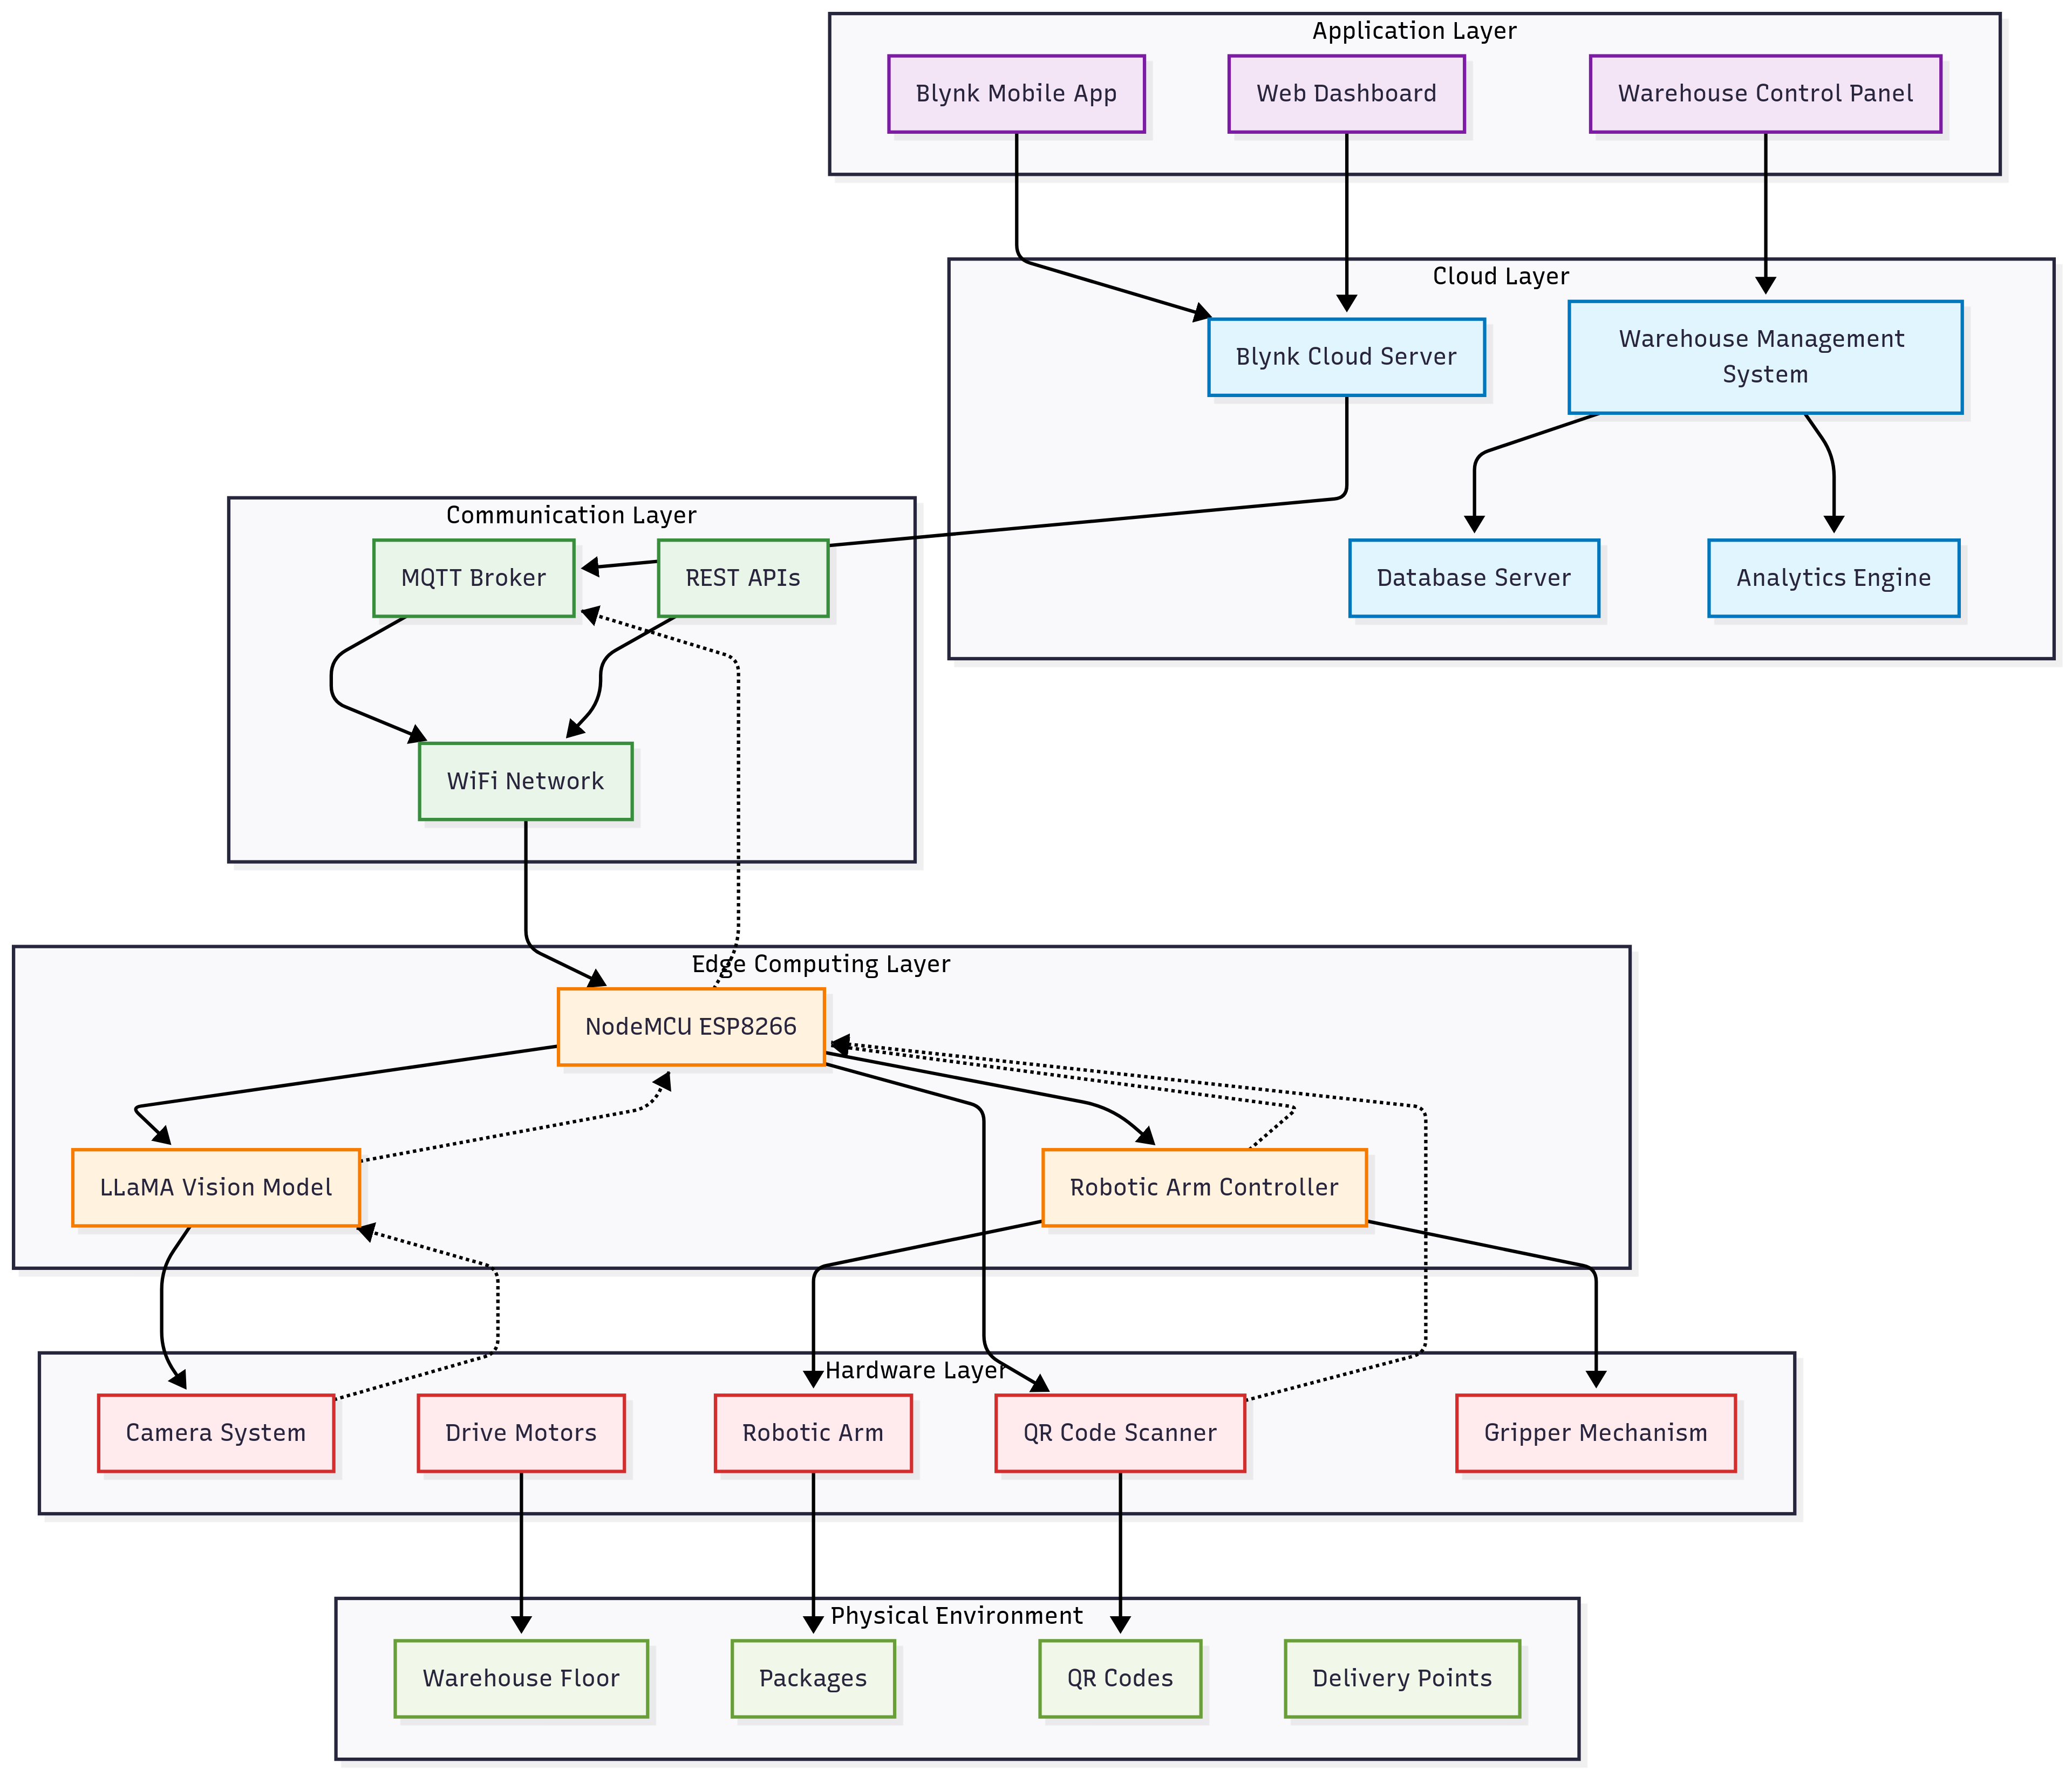
\includegraphics[width=0.9\textwidth]{./Chapter3/Figures/architecture-diagram.png}
    \caption{System Architecture of Autonomous Delivery Vehicle}
    \label{fig:architecture}
\end{figure}

\begin{verbatim}
NodeMCU ESP8266 (Central Controller)
├── L298N Motor Driver → DC Motors (Left/Right)
├── Servo Controllers → Robotic Arm (Base, Shoulder, Gripper)
├── Camera Module → Image Capture
├── Wi-Fi Module → Cloud Communication
└── Power Management → Battery/Charging System
\end{verbatim}

\subsection{Software Architecture Framework}
The software architecture implements a multi-threaded approach:

\begin{itemize}
\item \textbf{Main Control Thread}: Navigation logic and high-level decision making
\item \textbf{Motor Control Thread}: Real-time motor speed and direction control
\item \textbf{Arm Control Thread}: Precise servo positioning and gripper control
\item \textbf{Vision Processing Thread}: Image capture and QR code recognition
\item \textbf{Communication Thread}: Cloud data transmission and command reception
\end{itemize}

\subsection{Data Flow Architecture}
The system processes information through the following data flow:

\begin{enumerate}
\item \textbf{Sensor Input}: Camera captures environmental data and QR codes
\item \textbf{Processing}: Local preprocessing and cloud-based analysis
\item \textbf{Decision Making}: Navigation and manipulation commands generation
\item \textbf{Action Execution}: Motor and servo control for physical movement
\item \textbf{Feedback}: Status reporting and position updates to cloud system
\end{enumerate}

\section{Hardware Design Equations and Calculations}

\subsection{Motor Control Calculations}
The PWM-based speed control system uses the following relationship:

\begin{equation}
V_{motor} = V_{supply} \times \frac{PWM_{duty}}{255}
\end{equation}

Where:
\begin{itemize}
\item $V_{motor}$ = Effective motor voltage
\item $V_{supply}$ = Supply voltage (5V)
\item $PWM_{duty}$ = PWM duty cycle value (0-255)
\end{itemize}

\subsection{Robotic Arm Kinematics}
The forward kinematics for the 3-DOF arm is calculated using:

\begin{equation}
\begin{bmatrix}
x \\
y \\
z
\end{bmatrix}
=
\begin{bmatrix}
L_1 \cos(\theta_1) + L_2 \cos(\theta_1 + \theta_2) \\
L_1 \sin(\theta_1) + L_2 \sin(\theta_1 + \theta_2) \\
h_{base}
\end{bmatrix}
\end{equation}

Where:
\begin{itemize}
\item $L_1, L_2$ = Link lengths
\item $\theta_1, \theta_2$ = Joint angles
\item $h_{base}$ = Base height
\end{itemize}

\subsection{Power Consumption Analysis}
Total system power consumption is calculated as:

\begin{equation}
P_{total} = P_{ESP8266} + P_{motors} + P_{servos} + P_{camera} + P_{comm}
\end{equation}

Typical values:
\begin{itemize}
\item $P_{ESP8266}$ = 170mA @ 3.3V = 0.56W
\item $P_{motors}$ = 2 × 500mA @ 5V = 5W (maximum)
\item $P_{servos}$ = 3 × 200mA @ 5V = 3W
\item $P_{camera}$ = 100mA @ 5V = 0.5W
\item $P_{comm}$ = 80mA @ 3.3V = 0.26W
\end{itemize}

\section{Software Architecture and Implementation Strategy}

\subsection{Embedded Software Framework}
The embedded software utilizes a real-time operating system approach with the following modules:

\begin{itemize}
\item \textbf{Navigation Module}: Path planning and obstacle avoidance
\item \textbf{Vision Module}: Image processing and QR code decoding
\item \textbf{Manipulation Module}: Robotic arm control and gripper operations
\item \textbf{Communication Module}: Wi-Fi connectivity and cloud interface
\item \textbf{Safety Module}: Emergency stop and collision prevention
\end{itemize}

\subsection{Machine Learning Integration}
The LLaMA-4 model integration follows a hybrid approach:

\begin{enumerate}
\item \textbf{Local Processing}: Basic image preprocessing and QR code detection
\item \textbf{Cloud Analysis}: Complex object recognition and classification
\item \textbf{Edge Caching}: Frequently recognized objects stored locally
\item \textbf{Adaptive Learning}: Continuous model improvement based on operational data
\end{enumerate}

\subsection{State Machine Design}
The system operates using a finite state machine with the following states as depicted in Figure \ref{fig:state_machine}. The state machine provides a clear operational framework that ensures predictable behavior and efficient task execution.

\begin{figure}[H]
    \centering
    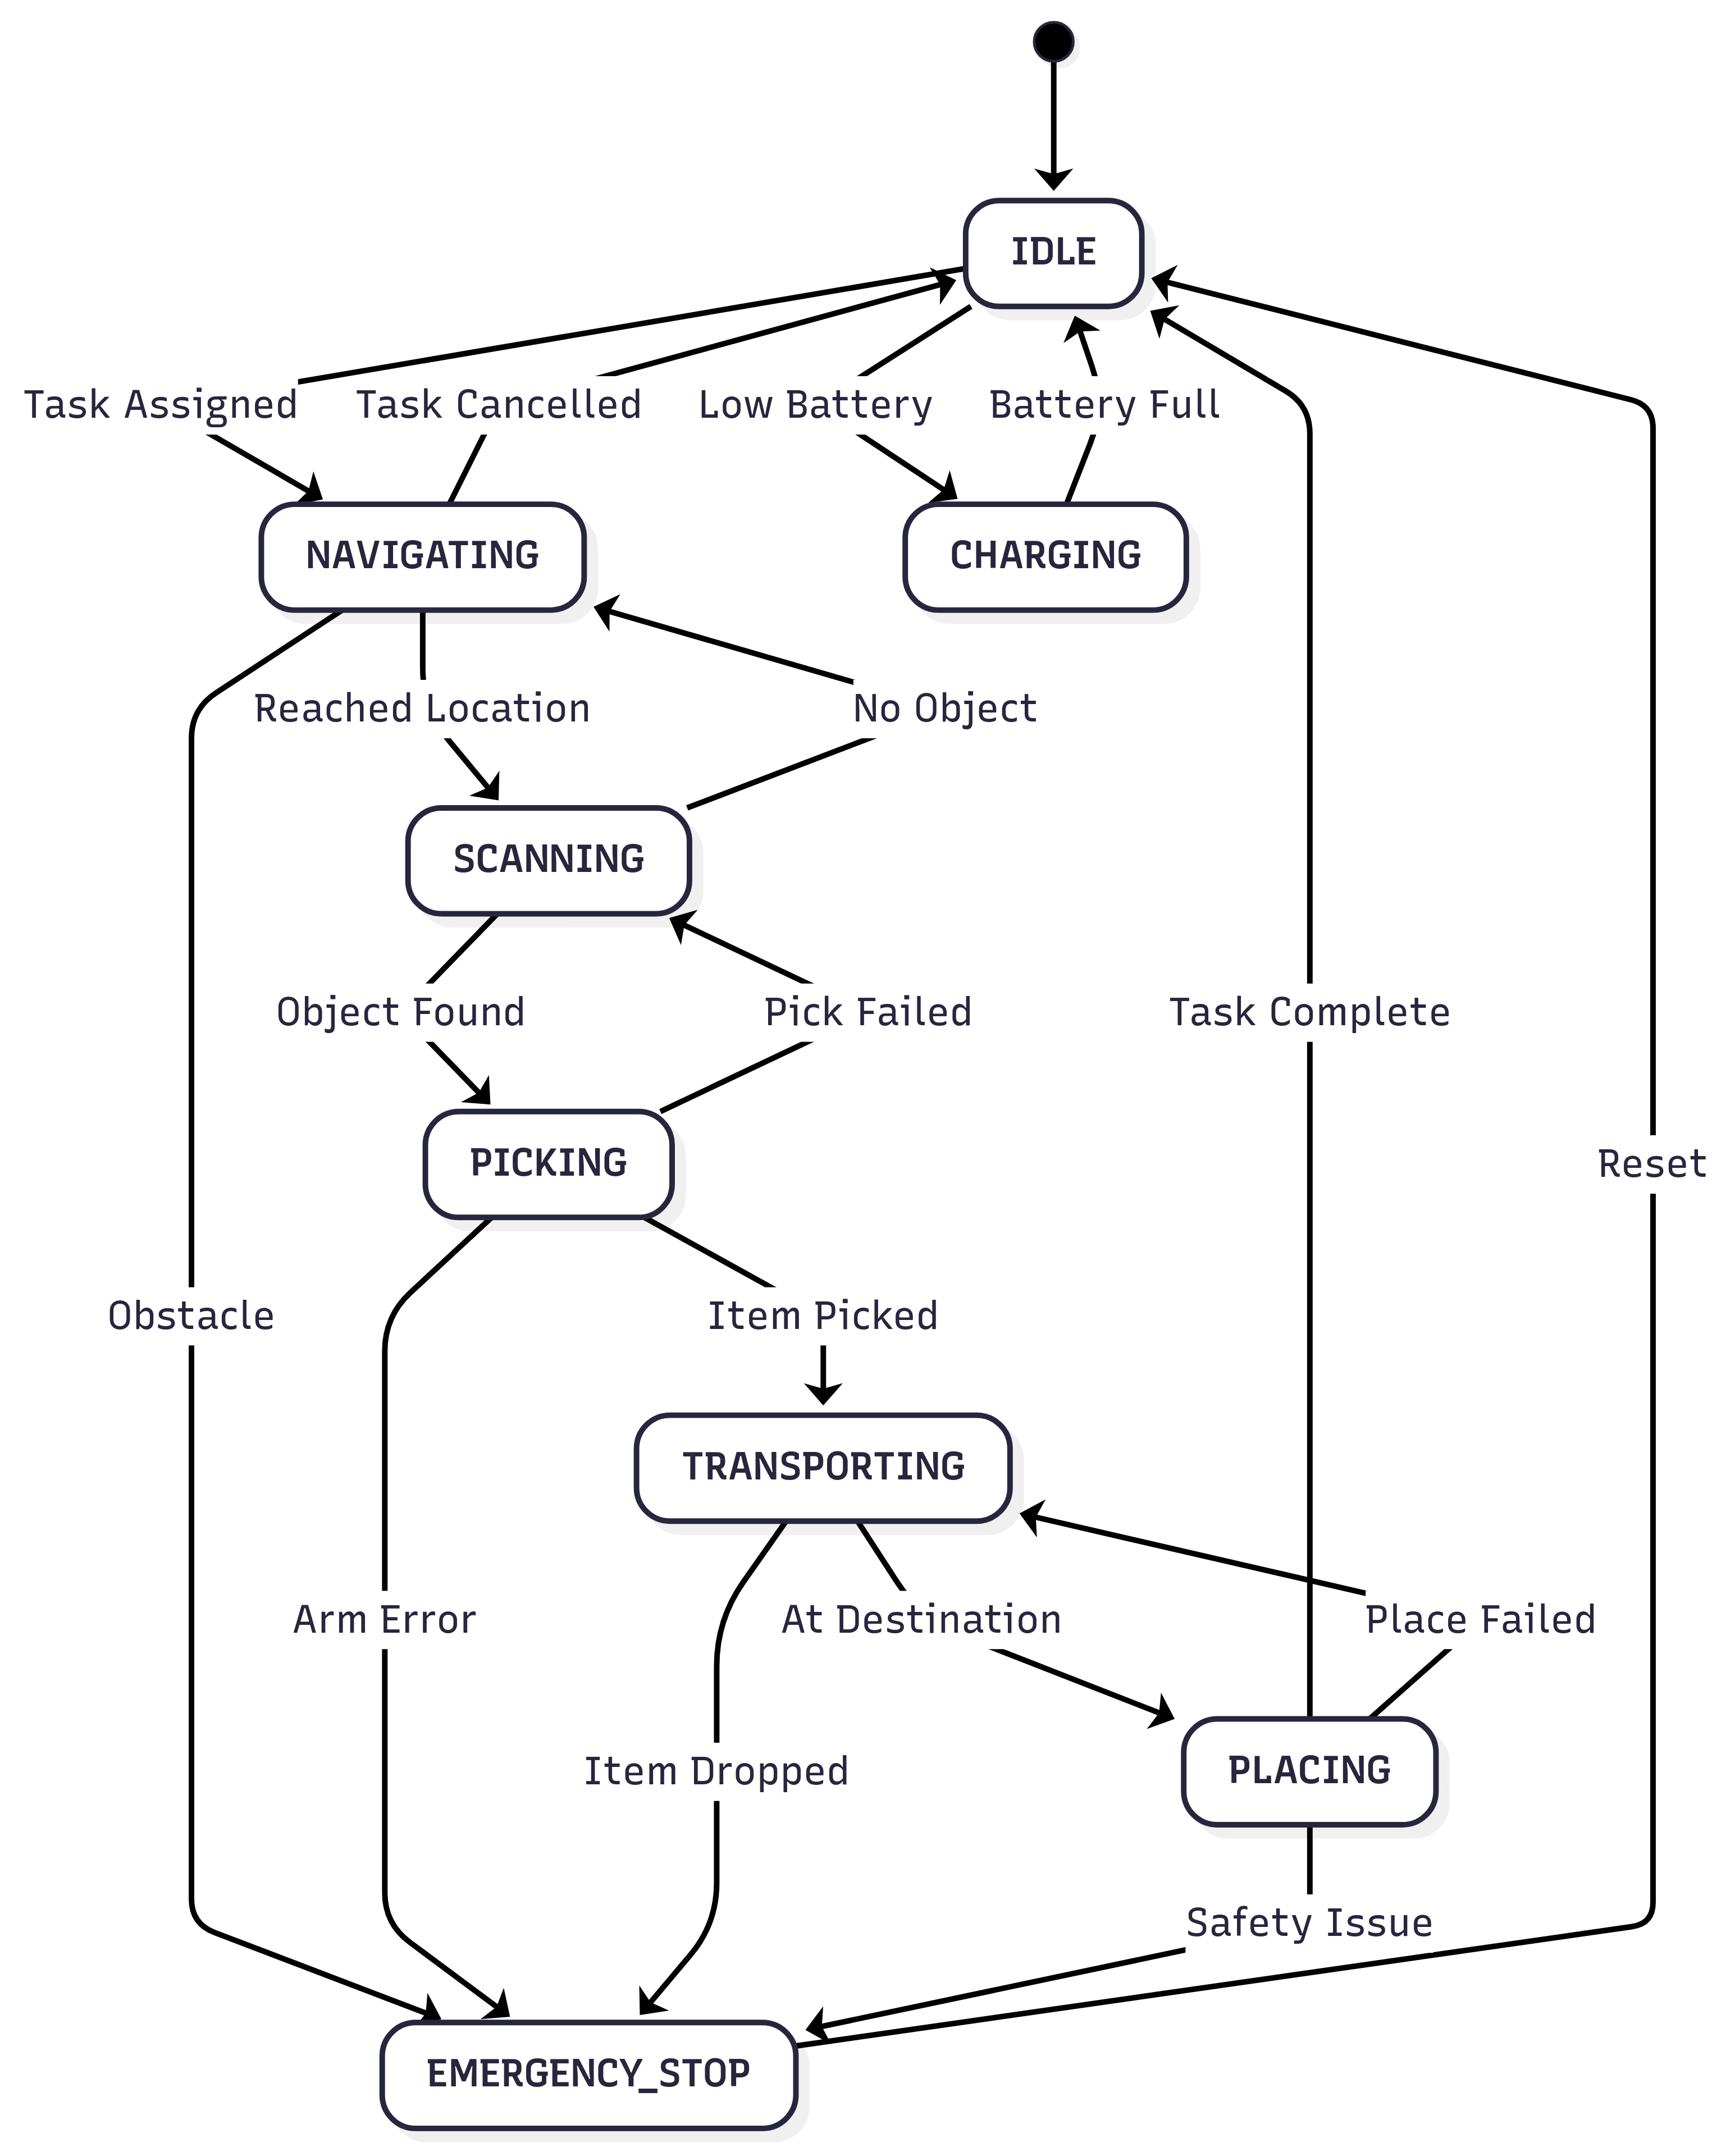
\includegraphics[width=0.8\textwidth]{./Chapter3/Figures/state-diagram.png}
    \caption{State Machine Diagram for Autonomous Delivery Vehicle}
    \label{fig:state_machine}
\end{figure}

\begin{itemize}
\item \textbf{IDLE}: Waiting for task assignment
\item \textbf{NAVIGATING}: Moving to target location
\item \textbf{SCANNING}: QR code recognition and object identification
\item \textbf{PICKING}: Robotic arm engagement and item retrieval
\item \textbf{TRANSPORTING}: Moving with payload to destination
\item \textbf{PLACING}: Item placement and task completion
\item \textbf{RETURNING}: Return to base or standby position
\end{itemize}

\section{Communication Protocol Design}

\subsection{Cloud Communication Architecture}
The system employs a RESTful API architecture for cloud communication:

\begin{itemize}
\item \textbf{HTTP/HTTPS}: Secure data transmission protocol
\item \textbf{JSON Format}: Lightweight data exchange format
\item \textbf{Real-time Updates}: WebSocket connections for live monitoring
\item \textbf{Command Interface}: Cloud-to-device control commands
\end{itemize}

\subsection{Data Transmission Protocol}
The communication protocol includes the following message types:

\begin{enumerate}
\item \textbf{Status Updates}: Position, battery level, task progress
\item \textbf{Sensor Data}: Camera images, QR code scans, environmental data
\item \textbf{Command Reception}: Task assignments, navigation updates
\item \textbf{Error Reporting}: System faults, maintenance requirements
\end{enumerate}

\subsection{QR Code Data Structure}
The QR code encoding follows a standardized format:

\begin{verbatim}
QR_CODE_DATA = {
    "location_id": "ZONE_A_SHELF_12",
    "coordinates": {"x": 45.2, "y": 23.8},
    "zone_type": "STORAGE",
    "access_level": "STANDARD",
    "timestamp": "2024-01-15T14:30:00Z"
}
\end{verbatim}

\section{Testing and Validation Methodology}

\subsection{Unit Testing Strategy}
Individual system components undergo rigorous testing:

\begin{itemize}
\item \textbf{Motor Control}: Speed accuracy, direction control, PWM response
\item \textbf{Servo Control}: Position accuracy, repeatability, response time
\item \textbf{Camera System}: Image quality, focus accuracy, lighting adaptation
\item \textbf{Communication}: Data transmission reliability, latency measurements
\end{itemize}

\subsection{Integration Testing Framework}
System-level testing validates complete functionality:

\begin{enumerate}
\item \textbf{Navigation Testing}: Path following accuracy, obstacle avoidance
\item \textbf{Pick and Place Testing}: Object handling reliability, precision
\item \textbf{Vision System Testing}: Object recognition accuracy, QR code reading
\item \textbf{End-to-End Testing}: Complete task execution validation
\end{enumerate}


\subsection{Performance Metrics}
Key performance indicators for system validation:

\begin{itemize}
\item \textbf{Task Completion Rate}: Percentage of successfully completed deliveries
\item \textbf{Position Accuracy}: Deviation from target positions (±5cm tolerance)
\item \textbf{Object Recognition Accuracy}: Percentage of correctly identified items
\item \textbf{System Uptime}: Continuous operation time before maintenance
\item \textbf{Battery Life}: Operating duration on single charge cycle
\end{itemize}